% Chapter Template

\chapter{X-ray luminosity - age relationship} % Main chapter title

\label{Chapter3} % Change X to a consecutive number; for referencing this chapter elsewhere, use \ref{ChapterX}
%----------------------------------------------------------------------------------------
%Commands
\newcommand{\Chandra}{\textit{Chandra}\xspace}
\newcommand{\XMM}{\textit{XMM-Newton}\xspace}
%----------------------------------------------------------------------------------------
%	SECTION 1
%----------------------------------------------------------------------------------------

\epigraph{\itshape There are only four rules you need to remember: make the plan, execute the plan, expect the plan to go off the rails, throw away the plan.}{---L. Snart, \itshape The Flash}

\section{Introduction}
The work presented in this chapter was published in the Monthly Notices of the Royal Astronomical Society, Volume 471, p.1012-1025 as the article entitled "An improved age-activity relationship for cool stars older than a gigayear" \citep{Booth_etal_2017} and modified here to fit within the framework and context of this thesis. This chapter discusses the work conducted in \citet{Booth_etal_2017} in greater depth. The aim of this study was to investigate the age-activity relationship beyond a gigayear using X-ray luminosity as a magnetic activity indicator and asteroseismology as the main source for stellar ages.

\subsection{Chandra and XMM-Newton telescopes}
This study utilises observations from both the \Chandra and \XMM X-ray telescopes which are space-based telescopes in highly eccentric orbits around Earth. This places the telescopes in an ideal position to perform long, uninterrupted observations that are necessary in the X-ray regime. It is worth mentioning that X-ray telescopes are unlike traditional optical telescopes in their setup. Since X-ray radiation passes through most material, the mirrors must be positioned almost parallel to the incoming photons. This causes the X-ray photons to reflect off the mirror at a grazing incidence, this process is repeated with a secondary mirror in order to focus the X-ray light to a focal point as shown in Figure \ref{fig:diagram_xray_telescope}.

\begin{figure}
    \centering
    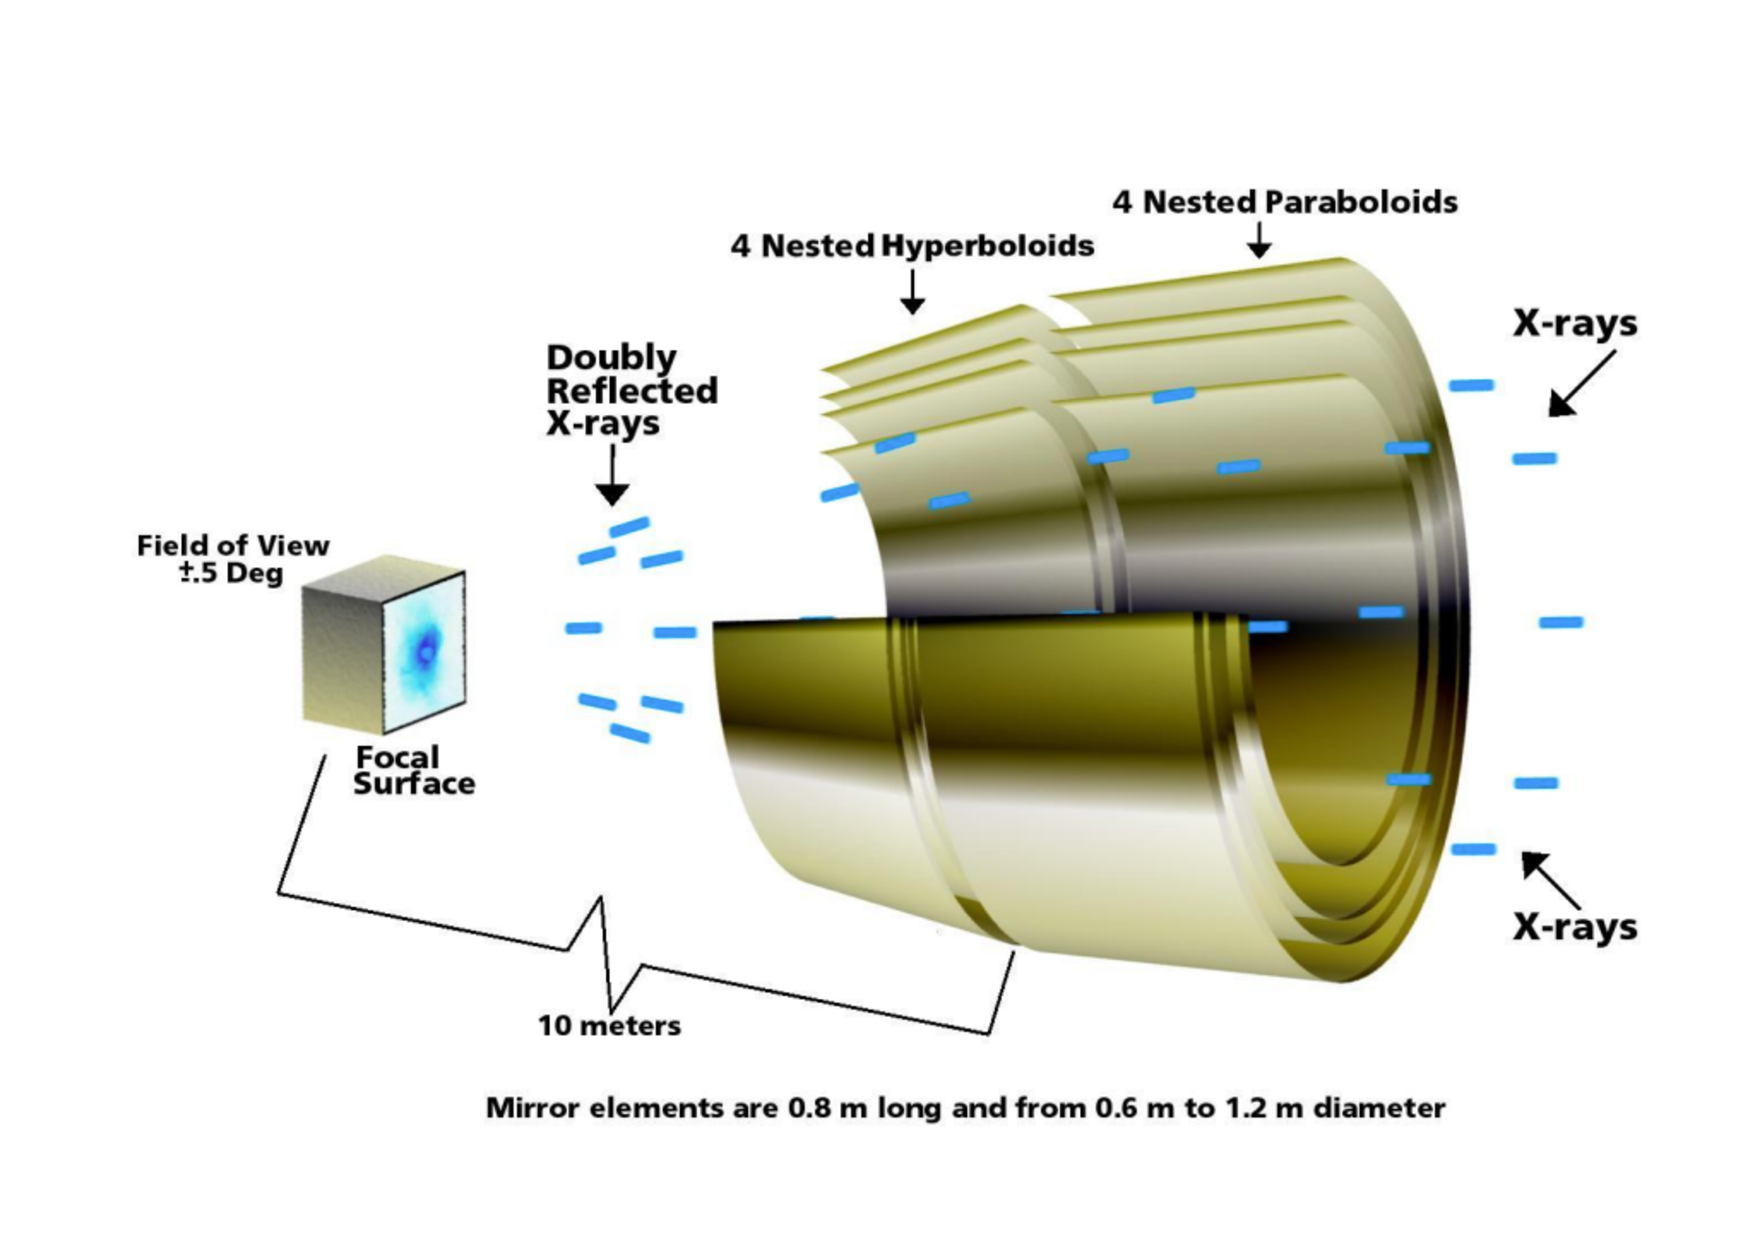
\includegraphics[scale=0.45]{Figures/3-Xray_age/chandra_scheme.pdf}
    \caption[Schematic of \Chandra X-ray telescope]{Schematic of \Chandra X-ray telescope. Four nested co-axial, confocal, grazing incident mirrors focus the X-ray photons to a common focal point where the detectors are located. Image Credit: NASA/CXC/ D. Berry}
    \label{fig:diagram_xray_telescope}
\end{figure}

The \XMM X-ray telescope \citep{Jansen_etal_2001} contains three X-ray CCD cameras collectively known as EPIC. EPIC is made up of one PN detector and two metal oxide detectors (MOS 1 and MOS 2). The MOS detectors are located behind the telescopes grating and only receives approximately half of the incident flux. Whereas the PN detector has an unobstructed beam and a much higher signal to noise than the MOS detectors, therefore data analysis is preferably performed with PN observations. The EPIC instrument is capable of imaging over the telescope's 30 arcmin field of view in the energy range 0.2 - 15 keV (62 - 0.826 \AA). Note that due to the short wavelengths of X-ray radiation, wavelengths are preferably presented in terms of energy. All of EPIC CCD's operate in a photon counting mode which produces an event list including the position of photon, arrival time and the photon energy; this allows for both imaging and spectra of X-ray objects to be obtined.

The \Chandra telescope \citep{Weisskopf_etal_2000} has two focal plane instruments: the advanced CCD imaging spectrometer (ACIS) and the high resolution camera (HRC). The HRC provides only images and no spectral information, therefore in this study observations are restricted to ACIS since it provides spectral information in the energy range 0.2 - 10 keV.

\section{Observations and stellar sample}
\subsection{Sample selection}
\label{Section_sample_selection}
Our target stars with well-determined ages were selected from several different sources. The majority stems from asteroseismology where stars were chosen with precisely determined stellar parameters, including ages, from modelling of individual oscillation frequencies as observed by the Kepler satellite \citep{Silva_Aguirre_etal_2015,Silva_Aguirre_etal_2017}. However, for some stars the signal to noise was not high enough to model the individual oscillation frequencies. In these circumstances, the global asteroseismic parameters \citep{Chaplin_etal_2014} were combined with spectroscopic parameters ($T_{eff}$ and [Fe/H]) \citep{Buchhave_Latham_2015} and ages are obtained through \texttt{BASTA} \citep{Silva_Aguirre_etal_2015}. \texttt{BASTA} uses a Bayesian approach to determine the probability that a set of parameters matches the observed asteroseismic parameters. Nearby stars were selected for dedicated X-ray observations with \XMM and \Chandra (PI: Poppenhaeger).

The second source is a sample of G and K type stars that are located in wide binaries with a white dwarf companion. As discussed in Section \ref{Section:intro_ages}, the ages of white dwarfs are relatively well known and can act as a stellar chronometer for the binary system. The binaries considered in this study are specifically wide binaries, this is to ensure that any binary companion has not gravitationally interacted with the main sequence star and altered its rotational (and thus magnetic activity) evolution. The sources for these systems are \citet{Garces_etal_2011} and \citet{Zhao_etal_2012}.

While ages have been derived for these systems by \citet{Garces_etal_2011}, more recent work into 3D models of white dwarfs showed that previous fits to 1D models overestimated the effective temperature and surface gravity \citep{Tremblay_etal_2013}. Therefore, a correction was applied to the effective temperatures and surface gravities calculated in \citet{Garces_etal_2011} by using Equations 7 and 8 from \citet{Tremblay_etal_2013}. With values for the effective temperature and surface gravity, the mass and cooling age of the white dwarfs were calculated using Montreal model grids for white dwarfs with hydrogen atmospheres\footnote{Available at \url{http://www.astro.umontreal.ca/~bergeron/CoolingModels/}} \citep{Holberg_Bergeron_2006,Kowalski_Saumon_2006,Bergeron_etal_2011,Tremblay_etal_2011}. However, to obtain the total age of the white dwarf, the initial-final mass relationship (Equation \ref{Eq:WD_init_final_relationship}) from \citet{Kalirai_etal_2008} was used which allows the mass of the progenitor star to be obtained. Padova stellar evolutionary models \citep{Bertelli_etal_2008} are then used to estimate the main sequence lifetime of the progenitor star which is added to the cooling age of the white dwarf to obtain the total age.

\begin{equation}
    M_{final} = 0.109M_{initial} + 0.394M_{\odot}
    \label{Eq:WD_init_final_relationship}
\end{equation}

The third source includes individually selected stars with archival X-ray observations and relatively well known ages through various methods. These age methods includes asteroseismology (16 Cyg A and B, $\alpha$ Cen / Promixa Cen system), isochrone fitting (61 Cyg A and B) and association with a subpopulation of stars in the galaxy (HR 7703). The Sun is also included in our sample and its age is taken to be $4.57 \pm 0.02$ Gyr \citep{Bahcall_etal_1995}. For the full details on the sample of stars used in this study and the various age methods used see Appendix \ref{App_lx_results}. One may wonder why Proxima Cen is included in this analysis as it is a fully convective star and previous discussion on the age-activity-rotation relationship was focused on stars with a stellar like dynamo (i.e. stars that have radiative core surrounded by a convective envelope). However, recent work by \citet{Wright_Drake_2016} considered a sample of fully convective stars and found that they follow an activity-rotation relationship that is indistinguishable to that of solar-type stars. Since the activity-rotation relationship is a well established proxy for the behaviour of the solar-like dynamo, this results suggest that these fully convective stars exhibit a solar-like dynamo and therefore it was included in the sample.

For stars with exoplanets in close orbits, effects on the stellar activity through star–planet interaction are expected from theoret- ical considerations \citep{Cuntz_etal_2000} and have been observed for some systems with high-mass exoplanets in very close orbits (see e.g. \citealt{Poppenhaeger_Wolk_2014,Pillitteri_etal_2015}). However, in our sample there are no stars with hot Jupiters present, therefore such effects are not expected to play a role in this investigation.

\subsection{Distances and spectral types}
\label{Section_Xray_distances_and_spectype}
It is known that the rotational evolution and thus the X-ray luminosity of stars no longer on the main sequence differ than those still on it, therefore only main sequence stars shoud be included in the sample. For several stars from the asteroseismic part of the sample, no luminosity classes were found in the literature. Therefore for these stars, their surface gravity (as calculated from asteroseismology) was compared to the relation of $B-V$ colour and surface gravity as given by \citet{Gray_2005} and shown in Equation \ref{Eq:Gray_2005}. Stars with surface gravities that differed by more than 0.2 dex of the value calculated by Equation \ref{Eq:Gray_2005} were excluded from the sample.

\begin{equation}
    \begin{aligned}
    \log(g) & = 4.25 - 0.3124(B-V) - 0.5022(B-V)^{2} + 6.532(B-V)^{3} \\
    &- 9.9431(B-V)^{4} + 5.7581(B-V)^{5} - 1.1706(B-V)^{6}
    \label{Eq:Gray_2005}
    \end{aligned}
\end{equation}

In order to determine the X-ray luminosity of a star, the distance is required. For the majority of the sample, distances were determined through parallaxes sourced from either SIMBAD \citep{Wenger_etal_2000} or \textit{Gaia} DR1 \citep{Gaia_Collaboration_2016_DR1}. For one star in the asteroseismic part of the sample, no distance or parallax was found in the literature. Therefore, for this star, the Barnes-Evans method was used to calculate the distance. The Barnes-Evans method uses a relation between angular diameter and V-K colour \citep{Fouque_Gieren_1997} shown in Equation \ref{Eq:Fouque_BE_relation} to calculate the angular diameter of a star ($\Theta$ - angular diameter in milli-arcseconds). Since the radius of the star is known through asteroseismology, this can be used with the angular diameter to determine the distance as shown in Equation \ref{Eq:distance_from_angular_diameter} which is derived from trigonometry where $\theta$ is the angular diameter in radians. Since the stars considered in this sample are all located relatively nearby then reddening was not taken into account. The Barnes-Evans method has been used previously to determine the stellar radii of exoplanet host stars and found good agreement with published values \citep{Watson_etal_2010}.

\begin{equation}
    \log\Theta = 0.5474 - 0.2V + 0.262(V-K)
    \label{Eq:Fouque_BE_relation}
\end{equation}

\begin{equation}
    d = \frac{2R_{*}}{\theta}
    \label{Eq:distance_from_angular_diameter}
\end{equation}

Finally, it was necessary to determine the spectral type of the candidates since this influences both the stellar activity and its evolution with time. The stellar spectral types were collected from the SIMBAD database \citep{Wenger_etal_2000}, or estimated from the stellar effective temperatures as published in \citet{Chaplin_etal_2014} and \citet{Silva_Aguirre_etal_2015}.

\section{Data analysis}
This section details the methods used to determine the X-ray luminosity for the sample of stars considered in this work.

Archival data for \XMM were obtained from the XMM-Newton Science Archive and analysed using \texttt{SAS} (Science Analysis system) version $15.0$. The data was filtered to remove any bad pixels or bad events by setting criteria to limit the probability of double photon impact events. This type of event occurs when two photons hit the same or neighbouring pixels in the same readout time frame and causes a slightly different pattern compared to a single photon event. For observations with \XMM, a standard source extraction radius of 20 arcsec was used and a source free background region was chosen with extraction radius of 70 arcsec. Data analysis was also preferably performed with PN observations due to the higher signal to noise from this instrument.

Archival observation files for \Chandra were obtained through the Chandra X-ray Centre public archive and analysed with \texttt{CIAO} (Chandra Interactive Analysis of Observations; \citealt{Fruscione_etal_2006}). For \Chandra data, a standard source extraction radius of 1.5 arcsec was used and a source free background region was chosen with radius of 15 arcsec. For a full list of X-ray observations see Table \ref{table:xray_obs_details}.

\begin{table}[t]
	\resizebox{\textwidth}{!}{
	\centering
	\begin{tabular}{lllc}
		\hline \hline
		Name of Star / White Dwarf & Telescope / Instrument     & Observation ID & Exposure Time / $10^{3}$ s \\
		\hline
		16 Cyg A & \Chandra ACIS-I  & 16647 & 35.33 \\
		 & \Chandra ACIS-I   & 18756 & 38.57 \\
		16 Cyg B & \Chandra ACIS-I  & 16647 & 35.33 \\
		 & \Chandra ACIS-I  & 18756 & 38.57 \\
		40 Eri A/40 Eri B & \Chandra ACIS-S  & 13644  & 5.00 \\
		61 Cyg A & \textit{XMM} PN Thick Filter & 41740301$^*$ & 7.09  \\
		61 Cyg B  & \textit{XMM} PN Thick Filter & 41740301$^*$  & 7.09 \\
		CD -3710500 / L481-60 & \Chandra ACIS-I   & 13769 & 24.75 \\
		GJ 176 & \Chandra ACIS-S  & 13638 & 4.98  \\
		GJ 191 & \Chandra ACIS-S   & 13646 & 5.00 \\
		HR 7703 & \textit{XMM} PN Thick Filter & 670380401 & 7.95  \\
		KIC 10016239 & \textit{XMM} PN Medium Filter & 761560601 & 22.24  \\
		KIC 12011630 & \Chandra ACIS-I HETG  & 9969 & 19.74 \\
		KIC 3123191 & \Chandra ACIS-I  & 13166 & 2.72 \\
		KIC 5309966 & \Chandra ACIS-I   & 17138 & 26.43 \\
		 & \Chandra ACIS-I  & 17141 & 29.69  \\
		 & \Chandra ACIS-I  & 17513 & 49.40 \\
		 & \Chandra ACIS-I  & 17516  & 49.02  \\
		KIC 6116048 & \textit{XMM} PN Medium Filter & 722330201 & 11.58 \\
		 & \textit{XMM} PN Medium Filter & 722330301 & 10.73 \\
		KIC 6603624 & \textit{XMM} PN Medium Filter & 761560701 & 35.67 \\
		KIC 7529180  & \textit{XMM} PN Thin Filter & 743460201 & 18.07 \\
		KIC 8292840 & \textit{XMM} PN Medium Filter & 743840201 & 10.74 \\
		KIC 9025370 & \textit{XMM} PN Medium Filter & 761560501 & 8.92 \\
		KIC 9410862 & \textit{XMM} PN Medium Filter & 670140501 & 26.36\\
		KIC 9955598 & \textit{XMM} PN Medium Filter & 761560601 & 22.24 \\
		NLTT 7887 / NLTT 7890 & \textit{XMM} PN Medium Filter & 670650101 & 16.60  \\
		Proxima Centauri & \textit{XMM} PN Medium Filter & 551120201$^*$ & 26.49 \\
		Alpha Centauri B & \textit{XMM} PN Thick Filter & 760290301$^*$ & 14.88 \\     
		\hline
		\end{tabular}}
		\caption[List of X-ray observations used in study]{Table of observations that were fully analysed and presented in the results Section. $^*$A large number of observations exist for these targets and has been taken into account in our analysis; one specific observation is listed to illustrative typical exposure times.}
		\label{table:xray_obs_details}
\end{table}

\subsection{Source detection}
For each target, the data was tested to see if a source was significantly detected in X-rays using the images from the observations. The number of X-ray counts were extracted from the source and background region in the 0.2 - 2.0 keV energy range as this is the region where weakly active cool stars emit most of their X-ray emission.

For \XMM data, there is typically a significant background signal detected in any observation. Therefore, the number of counts expected from a pure background  ($C_{0}$) was estimated by scaling the number of counts detected in the background region to the number expected in an area equivalent to the source region as shown in Equation \ref{Eq:C0_equation} where $C_{b}$ is the number of counts in the background region and $R_{b}$ and $R_{s}$ are the radii of the background and source regions, respectively. The number of counts in the source region ($C_{s}$) is then compared to the $C_{0}$ value and if it exceeds this value by $3\sigma$ then an X-ray source has been detected, otherwise an upper limit is calculated using the $3\sigma$ level over the background signal. Note that $\sigma$ is estimated to be the square root of the number of expected background counts ($C_{0}$). 

\begin{equation}
    C_{0} = \frac{C_{b}}{R_{b}^{2}}R_{s}^{2}
    \label{Eq:C0_equation}
\end{equation}

For \Chandra data, the background signal is typically very low meaning that estimating $\sigma$ as the square root of $C_{0}$ is invalid. Therefore, full Poisson statistics were used and the inverse per cent point function was calculated at which, for a given expected number of background counts (i.e. $C_{0}$), the number of counts in the source region had a probability of less than 0.3 per cent of occurring as a random fluctuation. If the number of source counts was greater than this value then the source was detected; otherwise, that number was used as the upper limit on the X-ray counts for the source. For both \Chandra and \XMM data, the fractional error on $C_{s}$ was taken to be $\frac{\sqrt{C_{s}}}{C_{s}}$.

\subsection{Stellar variability}
The typical exposure time for an X-ray observation is on the order of 10 ks ($\approx$ few hours), however, stars can have variability that occurs on shorter time-scales than this. Therefore, for detected target stars, a light curve was extracted from each observation to check for short-term magnetic phenomena such as flares. This is important as flares release a large amount of energy which causes the corona to heat up thus increasing the temperature and emission measure of the corona (emission measure simply means the amount of material that emits at a particular temperature and is used in spectral fitting - see Section \ref{Section_Determining_Xray_flux}). If flares are detected in our observations, it can result in a significantly higher X-ray luminosity than the quiescent emission level of the star.

\begin{figure}
    \centering
    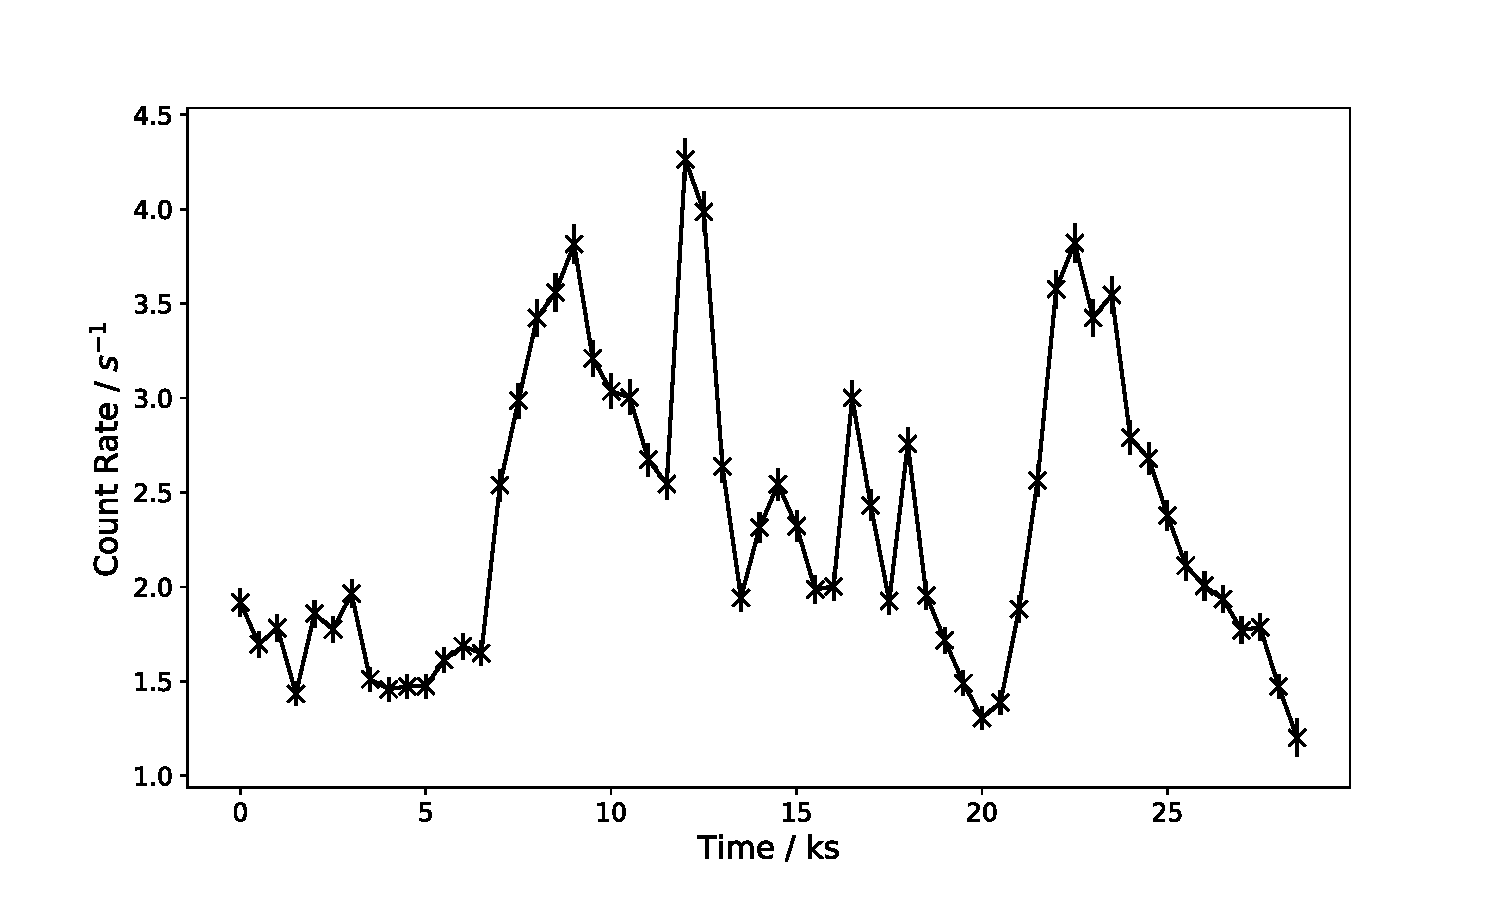
\includegraphics[scale=0.5]{Figures/3-Xray_age/proxima_cen_lc.pdf}
    \caption[X-ray light curve of Proxima Centauri]{X-ray light curve of Proxima Centauri. This plot shows the count rate during the observation and would suggest that several flares occurred during this time.}
    \label{fig:proxima_cen_lc}
\end{figure}

\begin{figure}
    \centering
    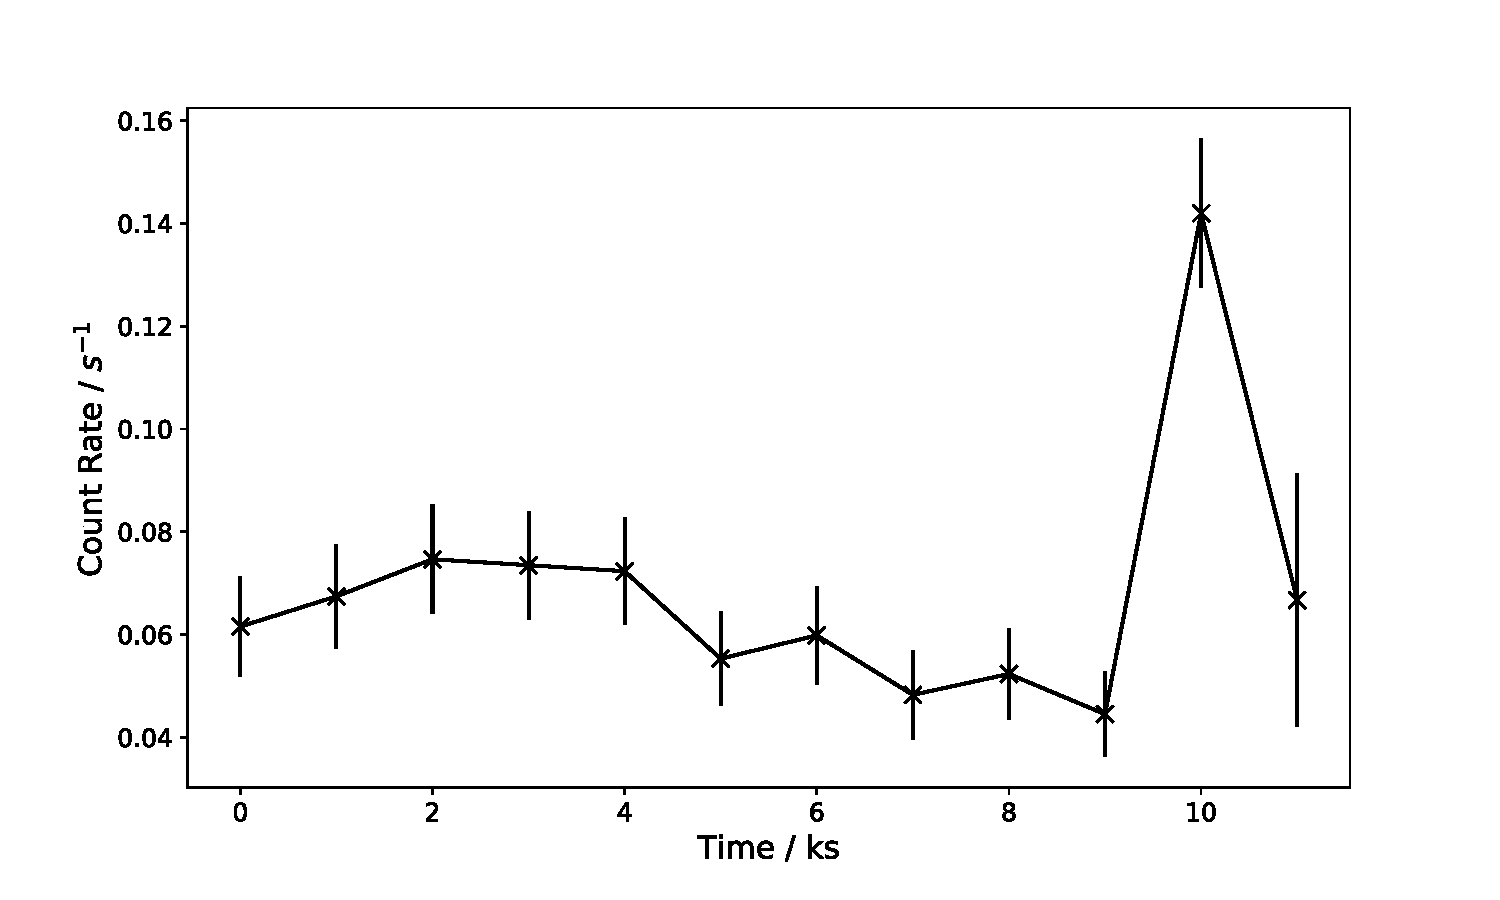
\includegraphics[scale=0.5]{Figures/3-Xray_age/HR7703_lc.pdf}
    \caption[X-ray light curve of HR 7703]{X-ray light curve of HR 7703. This plot shows the count rate during the observation and would suggest that a flare occurred towards the end of this observation.}
    \label{fig:HR7703_lc}
\end{figure}

In the case of Proxima Centauri, the light curve showed several rapid increases in the count rate over the observation exposure time, indicating several flares as shown in Figure \ref{fig:proxima_cen_lc}. Therefore, the quiescent value for the X-ray luminosity of $4.9 \times 10^{26}$ erg $s^{-1}$ was taken from \citet{Fuhrmeister_etal_2011} and used in this work. An inspection of the light curve for HR 7703 indicated that a flare had occurred towards the end of the observation as shown in Figure \ref{fig:HR7703_lc}. In this case, the time interval associated with the flare was excluded from the data analysis.

\subsection{Determining the X-ray flux}
\label{Section_Determining_Xray_flux}
For X-ray sources with significant detections and where the source region contained $\approx 90$ or more counts, the spectra of the source was modelled with a coronal plasma model in order to determine the X-ray flux. A spectrum for the star was extracted from the observations using the relevant analysis tools for each telescope. Using the \texttt{XSPEC} fitting software, the extracted spectra were fitted with an optically thin thermal plasma model (APEC model). The APEC model has four parameters: coronal temperature (keV), metal abundances, redshift and norm. The last parameter, norm ($\eta$), is a distance scaled emission measure (EM) of the gas and is defined by Equation \ref{Eq:norm_parameter_apec_model} where $D_{A}$ is the angular diameter distance to the source in centimetres. The emission measure is defined as a measure of the amount of material that is emitting at a certain temperature and is defined by Equation \ref{Eq:EM_parameter} where $n_{e}$ and $n_{H}$ are the electron and Hydrogen densities. Since all of the stars considered in this sample are located nearby then the redshift was fixed at zero; the abundances were assumed to be solar by using abundances from \citet{Grevesse_Sauval_1998}. Using solar abundances is a reasonable approximation for fairly low-resolution spectra as no significant spectral features are resolved that are highly dependent on metallicity abundances. \textcolor{red}{Check the reason with Katja}
Therefore, the two parameters that were fitted were coronal temperature and norm; in some cases, two temperature components were required to find a suitable fit for the coronal spectrum. The \texttt{XSPEC} fitting software uses a modified Levenberg-Marquardt algorithm to minimise the fit statistic and is based on \texttt{CURFIT} from \citet{Bevington_1969}. However, the Levenberg-Marquardt algorithm only finds the local minimum which is not necessary the global minimum, therefore, the initial conditions for each parameter that is to be fitted must be reasonable guesses. From the best-fitting model to each object, the flux was then calculated in a fixed energy band from 0.2 to 2 keV. The details and plots of the best-fitting models are shown in Table \ref{table:spectral_fit_details} and Appendix \ref{Appendix_Xray_spectra}, respectively

\begin{equation}
    \eta = \frac{1 \times 10^{-14} \text{EM}}{4\pi(1+z)^{2}D_{A}^{2}}
    \label{Eq:norm_parameter_apec_model}
\end{equation}

\begin{equation}
    \text{EM} = \int n_{e}n_{H} dV
    \label{Eq:EM_parameter}
\end{equation}


\begin{table}
\centering
\begin{tabular}{l c c c}
	\hline \hline
	Name of Star & Model kT & Model Emission Measure  & Reduced chi-squared\\
    & (keV)          &($\frac{4\pi d^2}{10^{-14}}$ cm$^{-3}$) & \\
	\hline
	40 Eri A & 0.19 & $9.9\times 10^{-5}$ & 1.59\\
	CD -3710500 & 0.44 & $2.2\times 10^{-4}$ & 0.32\\
	GJ 176 & 0.37 & $3.4\times 10^{-5}$ & 1.49\\
	GJ 191 & 0.30 & $5.4\times 10^{-5}$ & 2.52\\
	HR 7703 & 0.17 & $5.31\times 10^{-5}$ & 1.34\\
	& 0.76 & $1.45\times 10^{-5}$  &\\
	KIC 7529180 & 0.22 & $9.8\times 10^{-6}$ & 1.70\\
	& 0.91 & $1.7\times 10^{-5}$  &\\
	61 Cyg A & 0.21 & $4.09\times 10^{-4}$ & 1.99\\
	& 0.79 & $1.75\times 10^{-4}$  &\\
	61 Cyg B & 0.19 & $1.71\times 10^{-4}$ & 1.17\\
	& 0.67 & $5.06\times 10^{-4}$  &\\
	\hline
	\end{tabular}
	\caption[X-ray spectral modelling results]{Best-fitting model parameters used to calculate the X-ray flux between 0.2 and 2.0 keV for stars that were sufficiently detected in X-rays.}
	\label{table:spectral_fit_details}
\end{table}

In the case where the source region contained $\approx$ 90 counts or less, then typically there were not enough data points to fit a spectrum accurately. Therefore, an estimate of the X-ray flux was obtained through WebPIMMS\footnote{\url{https://heasarc.gsfc.nasa.gov/cgi-bin/Tools/w3pimms/w3pimms.pl}} using the mean count rate of the source region. A typical spectrum was assumed for the stellar corona, and WebPIMMS calculated the source flux using the instrument characteristics. The X-ray flux was calculated in the $0.2 - 2.0$ keV energy range assuming an APEC model of solar abundance and $\log T$ value of 6.5 ($T \approx 3$ MK), appropriate for inactive cool stars. The conversion factors from counts to flux used for each of the instruments are shown in Table \ref{table:webpimms_conversion_factors}; note that the sensitivity of \Chandra changes significantly over the years of operation, and therefore the correct conversion factors need to be chosen for the observing cycle in which a given observation took place. For \XMM observations, the encircled energy fraction factor needs to be applied as well since its point spread function (PSF) is significantly larger than typical source extraction radii. Since a 20 arcsec source radius, this encloses approximately 80\% of the PSF and thus any count rates observed were corrected by dividing by $0.8$.

\begin{table}
	\centering
	\begin{tabular}{l c}
		\hline \hline
		Name of Instrument & Conversion Factor \\
         & (erg s$^{-1}$ cm$^{-2}$ count$^{-1}$) \\ 
		\hline
		XMM PN Medium Filter & $1.03\times10^{-12}$\\
		Chandra ACIS-I No Grating (Cycle 16) & $2.42\times10^{-11}$\\
		Chandra ACIS-I No Grating (Cycle 12) & $1.52\times10^{-11}$\\
		Chandra ACIS-I HET Grating (Cycle 10) & $2.16\times10^{-10}$\\
		\hline
	\end{tabular}
	\caption[Conversion factors used by WebPIMMS]{Conversion factors used by WebPIMMS to convert number of counts into flux in the $0.2 - 2.0$ keV energy range, assuming a coronal temperature of $\log T = 6.5$ and solar abundances.}
	\label{table:webpimms_conversion_factors}
\end{table}

The statistical error on the values of X-ray counts was calculated from the square root of the number of source counts ($C_{s}$) (as the distribution is described by Poisson statistics) and divided by the number of source counts to obtain a fractional error. This fractional error on the number of counts was also used as the error on the X-ray flux and the X-ray luminosity. However, the X-ray luminosity of a star is known to vary on various time-scales, including time-scales much shorter than the star’s main-sequence lifetime, therefore a minimum physical error of 0.1 dex in $\log L_{x}$ was applied to the data to account for this variability, even if the statistical error was smaller. This value was determined from the long-term X-ray monitoring of 61 Cyg B \citep{Robrade_etal_2012}, a star without an apparent activity cycle, where the standard deviation of the X-ray luminosity was at 0.1 dex over several years of observations. In order to convert X-ray flux into X-ray luminosity, Equation \ref{Eq:flux_luminosity} was used.

\begin{equation}
    L_{x} = 4\pi d^{2}F_{x}
    \label{Eq:flux_luminosity}
\end{equation}

\subsection{Additional notes on analysis}
In the previous section, the general methodology used to determine the X-ray luminosity is detailed. However, since the sample is made up of a number of observations from both the \XMM and \Chandra telescopes, additional details are presented here about the individual observations used and the data reduction.

\textit{16 Cyg A}: This star was detected by combining two \Chandra observations on a front-illuminated CCD, which only provides energy sensitivity above 0.6 keV. The flux was extrapolated for the full $0.2 - 2.0$ keV band by using WebPIMMS and assuming a coronal temperature of $\log T = 6.5$. The star 16 Cyg B was covered by the same observations, but is undetected and an upper limit is calculated. There is also an earlier, shorter \XMM observation covering both stars, but they were both undetected in that observation, which is consistent with the \Chandra data.

\textit{40 Eri A}: This star is in a wide binary system with the white dwarf 40 Eri B, with a projected distance of 83 arcsec \citep{Wenger_etal_2000}, translating to a physical distance of ca. 400 AU. Using the techniques outlined in Section \ref{Section_sample_selection}, its reported $T_{eff}$ and $\log g$ values \citep{Zhao_etal_2012} were used to calculate an age of $3.70^{+3.57}_{-1.34}$ Gyr for 40 Eri B, which is adopted as the age of the system. 40 Eri A was observed with a back-illuminated \Chandra CCD, which provides energy sensitivity above 0.245 keV. A spectral fit was performed and the X-ray flux was extrapolated for the full $0.2 - 2.0$ keV energy range. There is also a third star, 40 Eri C, present in the system; however, it is close enough to the white dwarf (ca 35 AU) that its rotation and activity properties may have been affected during the evolution of the white dwarf progenitor, which is why 40 Eri C is not included in the analysis.

\textit{61 Cyg A and B}: These stars have been monitored in X-rays with \XMM over several years. One exemplary X-ray spectrum for each star is shown in Figure \ref{App_A_61Cyg}. 61 Cyg A has been found to display an activity cycle \citep{Robrade_etal_2012}, and the full range of observed X-ray luminosities have been adopted as the error bar for 61 Cyg A's X-ray luminosity found in this work. 61 Cyg B has found to have a flat activity profile \citep{Robrade_etal_2012}, and the mean X-ray luminosity is adopted in this analysis with the standard deviation over all X-ray observations as the error on this value.

\textit{CD-3710500}: This star is in a wide binary system with the white dwarf L481-60. Using the techniques outlined in Section \ref{Section_sample_selection}, its reported $T_{eff}$ and $\log g$ values \citep{Zhao_etal_2012} were used to calculate an age of $1.77^{+0.65}_{-0.27}$ Gyr for L481-60, which is adopted as the age for the system. The star CD-3710500 was observed with a front-illuminated \Chandra CCD, which provides energy sensitivity above 0.6 keV. A spectral fit was performed and the X-ray flux was extrapolated for the full $0.2 - 2.0$ keV energy range.

\textit{GJ 176}: This star was detected with a back-illuminated \Chandra CCD, which provides energy sensitivity above 0.245 keV. A spectral fit was performed and the X-ray flux was extrapolated for the full $0.2 - 2.0$ keV energy range.

\textit{GJ 191}: This star was detected with a back-illuminated \Chandra CCD, which provides energy sensitivity above 0.245 keV. A spectral fit was performed and the X-ray flux was extrapolated for the full $0.2 - 2.0$ keV energy range. The X-ray luminosity found is consistent with the values reported by \citet{Guinan_etal_2016}.

\textit{HR 7703}: This source was detected with \XMM and a spectral fit was performed for the full energy range of $0.2 - 2.0$ keV.

\textit{KIC 12011630, KIC 3123191 and KIC 5309966}: These stars were in the field of view of \Chandra during observations of other targets and are all undetected in X-rays. The sources are located on front-illuminated CCD's and are far from the centre of the field of view. Since \Chandra's PSF becomes large at the edges of the field of view, large extraction regions had to be used, which led to quite high upper limits for the X-ray luminosities for these stars.

\textit{KIC 10016239 and KIC 7529180}: These stars were detected with \XMM. KIC 7529180 was detected with a sufficient number of source counts so that a spectral fit could be performed. For KIC 10016239, the excess source counts were used to calculate the X-ray flux through WebPIMMS, assuming a coronal temperature of $\log T = 6.5$.

\textit{KIC 6116048, KIC 6603624, KIC 8292840, KIC 9025370, KIC 9410862}: These stars were observed with \XMM, but undetected in X-rays.

\textit{KIC 9955598}: This star was observed and detected with \XMM. Since there is another X-ray source at close projected distance (ca.\ $20$ arcsec), we chose an extraction region with a radius of $10$ arcsec instead of $20$ arcsec, and applied the correct encircled energy fraction factor (0.6) to account for the smaller extraction region when calculating the flux.

\textit{NLTT 7887}: This star is in a wide binary system with the white dwarf NLTT 7890. Since the reported surface gravity of the white dwarf has large errors \citep{Garces_etal_2011}, the age derived has large errors as well with $4.97^{+8.8}_{-3.0}$~Gyr. The star NLTT 7887 was covered by an \XMM observation, but is undetected.

\textit{$\alpha$ Cen A, $\alpha$ Cen B, Proxima Cen}: The age of this triple system has been derived from asteroseismic observations of $\alpha$ Cen A and $\alpha$ Cen B using different underlying models \citep{Miglio_Montalban_2005}; the mean of the asteroseismic age estimates has been adopted as the age of the system. $\alpha$ Cen A and $\alpha$ Cen B have been monitored in X-rays with \XMM \citep{Robrade_etal_2012}. $\alpha$ Cen B was found to display an activity cycle, and the full range of observed X-ray luminosities is used as the error bar on its X-ray luminosity for our analysis. $\alpha$ Cen A is reported by the same authors to potentially be in an activity cycle as well, however only the low-activity part has been observed so far, and there is no information on what its X-ray luminosity might be during the high-activity part of the cycle. Therefore $\alpha$ Cen A has not been included in this analysis. Proxima Cen has been observed with \XMM several times as well, including multiple stellar flares; a detailed analysis is given by \citet{Fuhrmeister_etal_2011}. Their quiescent X-ray luminosity of $\log L_{\mathrm{X}} = 26.69$ for Proxima Cen has been adopted in this analysis due to the number of flares seen in the observation (see Figure \ref{fig:proxima_cen_lc}).

\textit{Sun}: \citet{Peres_etal_2000} determined model parameters for the Sun in the 0.1 - 3.0 keV energy range to aid the interpretation of stellar coronae data. For this study, these parameters were adapted by using the reported values in \citet{Peres_etal_2000} and generating a model spectrum using the \texttt{XSPEC} fitting software. Specifically, the emission measure values for the Sun at maximum and minimum reported in Table 2 of \citet{Peres_etal_2000} were converted into norm ($\eta$) values using Equation \ref{Eq:norm_parameter_apec_model}. Note that in \citet{Peres_etal_2000}, a distance for the Sun was assumed to be 1 pc. The norm parameters were used in conjunction with the coronal temperatures reported in \citet{Peres_etal_2000} to generate a model spectrum in \texttt{XSPEC}. This model was then used to calculate the flux in the 0.2 - 2.0 keV energy range (to be consistent with the rest of the stellar sample) and converted to an X-ray luminosity. The age of the Sun was adopted to be $4.57 \pm 0.02$ Gyr \citep{Bahcall_etal_1995}.

\section{Results}
\subsection{Magnetic activity across spectral types}
It is known that there is a mass dependence on the rotational spin-down of late-type stars, as many rotational studies include a colour term as a proxy for mass (e.g. \citealt{Barnes_2003,Barnes_2010,Angus_etal_2015}). This is due to the varying depth of the convection zone, F stars have a much thinner convection zone which results in rotational spin-down that occurs on a different timescale than M dwarfs that have a much thicker convection zone. This mass dependence seen in the rotational spin-down will also be present in the evolution of X-ray luminosity with time across varying spectral types. Since the sample of stars considered in this work is relatively small, splitting the sample into different spectral types is non-ideal and an analysis of the whole sample is preferable.

When dealing with X-ray luminosity as a magnetic activity indicator, some studies normalise $L_{x}$ by the stellar bolometric luminosity and then split into different mass bins \citep{Preibisch_Feigelson_2005,Jackson_etal_2012}. However, a different approach was taken by \citet{Schmitt_Liefke_2004}; in their volume complete sample of cool stars in the solar neighbourhood, it was found that when the X-ray luminosity is divided by the stellar surface area $4\pi R_{*}^{2}$ with $R_{*}^{2}$ being the stellar radius, i.e. when one considers the X-ray flux through the stellar surface as a quantity of interest, then stars of all spectral types from F to M show the same spread in this quantity. We visualise these various quantities in Figure \ref{fig:Lx_normalise_schmitt_data}. The stars from \citet{Schmitt_Liefke_2004} were used to plot X-ray luminosity as a function of absolute stellar brightness as a proxy for stellar mass. Preference was given to data collected with the PSPC detector without the Boron filter if several observations were reported in \citet{Schmitt_Liefke_2004}(\textcolor{red}{Explain why}). Using "A Modern Mean Dwarf Stellar Color and Effective Temperature Sequence"\footnote{\url{http://www.pas.rochester.edu/~emamajek/EEM_dwarf_UBVIJHK_colors_Teff.txt}} \citep{Pecaut_Mamajek_2013}, the reported spectral types \citep{Schmitt_Liefke_2004} were used to find estimates for the effective temperature ($T_{eff}$) and bolometric magnitude ($M_{BOL}$). The bolometric magnitude was then used to calculate the bolometric luminosity using Equation \ref{Eq:bolometric_luminosity} where $L_{BOL\odot}$ is the solar bolometric luminosity ($3.827 \times 10^{33}$ erg s$^{-1}$) and $M_{BOL\odot}$ is the solar bolometric magnitude ($4.7554$). The stellar radius was calculated using Equation \ref{Eq:stellar_radius} where $k$ is the Boltzmann constant and has a value of $5.6704 \times 10^{-5}$ erg cm$^{-2}$ s$^{-1}$ K$^{-4}$. 

\begin{equation}
    L_{BOL} = L_{BOL\odot} 2.5^{M_{BOL\odot} - M_{BOL}}
    \label{Eq:bolometric_luminosity}
\end{equation}

\begin{equation}
    L_{BOL} = 4\pi R_{*}^{2}kT_{eff}^{4}
    \label{Eq:stellar_radius}
\end{equation}

Figure \ref{fig:Lx_normalise_schmitt_data} shows the comparison between X-ray luminosity, X-ray luminosity normalised by stellar surface area and X-ray luminosity normalised by bolometric luminosity. In the left panel of Figure \ref{fig:Lx_normalise_schmitt_data}, the intrinsic mass dependency of X-ray luminosity as a function of mass is clearly seen with higher mass stars typically being more active than lower mass stars. In the right panel of Figure \ref{fig:Lx_normalise_schmitt_data}, the X-ray luminosity normalised by the bolometric luminosity is shown; this shows that lower mass stars typically have higher values on this activity scale, opposite to the trend seen in the X-ray luminosity. This is most likely due to the dependency of bolometric luminosity on both the stellar radius and effective temperature (see Equation \ref{Eq:stellar_radius}), where the extreme differences in effective temperatures from F to M dwarfs causes the trend shown here. Whereas, if the X-ray luminosity through the stellar surface area is considered (as shown in the middle panel of Figure \ref{fig:Lx_normalise_schmitt_data}), a flat distribution is seen as a function of absolute magnitude (the proxy for mass in this plot) as reported by \citet{Schmitt_Liefke_2004}.

\begin{figure}
    \centering
    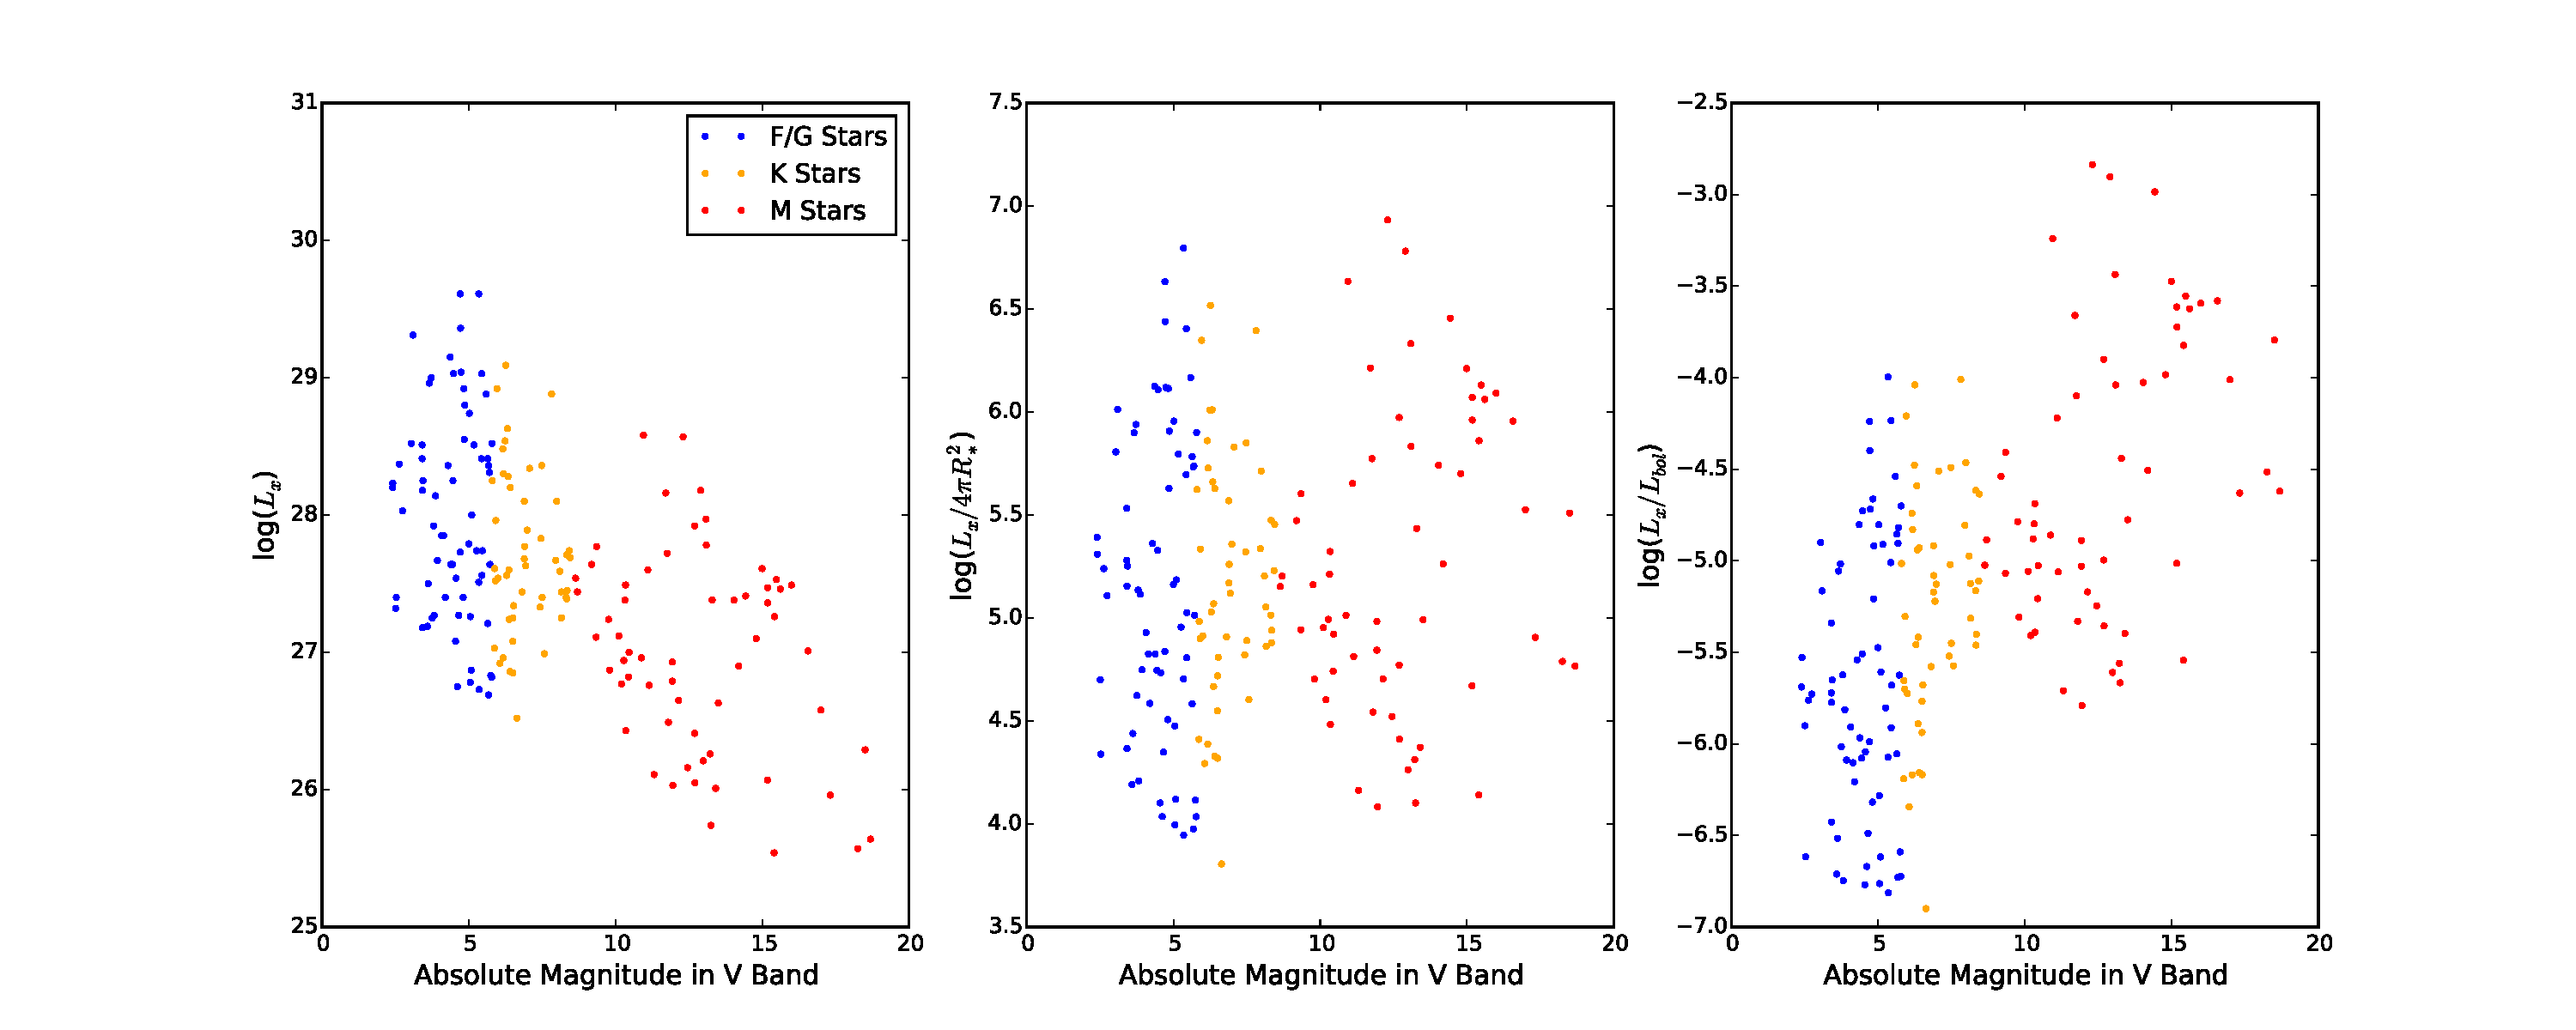
\includegraphics[scale=0.33]{Figures/3-Xray_age/normalise_schmitt_data.pdf}
    \caption[Comparison of X-ray luminosity and normalised parameters]{Comparison of data taken from \citet{Schmitt_Liefke_2004} when normalised by bolometric luminosity and stellar surface. \textbf{Left Panel}: Logarithmic value of X-ray luminosity as a function of absolute magnitude in V band. \textbf{Middle Panel}: Logarithmic value of X-ray luminosity normalised by the stellar surface area as a function of absolute magnitude in V band. \textbf{Right Panel}: Logarithmic value of the ratio of X-ray luminosity to bolometric luminosity as a function of absolute magnitude in V band.}
    \label{fig:Lx_normalise_schmitt_data}
\end{figure}

Therefore, the X-ray luminosities of the sample of cool, inactive stars considered in this work were normalised by the stellar surface area as this allowed for a combined analysis of the full sample to be performed. The stellar radii for the stars in the sample were taken either from asteroseismology or calculated using the same technique described previously for the \citet{Schmitt_Liefke_2004} sample using absolute brightness and effective temperature.

\subsection{Fitting the data}
In total, 24 stars were fully analysed and are shown in Figure \ref{fig:Xray_sample}; the full details of the result for each star and stellar properties are listed in Appendix \ref{App_lx_results} and \ref{App_Xray_sample_stellar_properties}, respectively. 

\begin{figure}
    \centering
    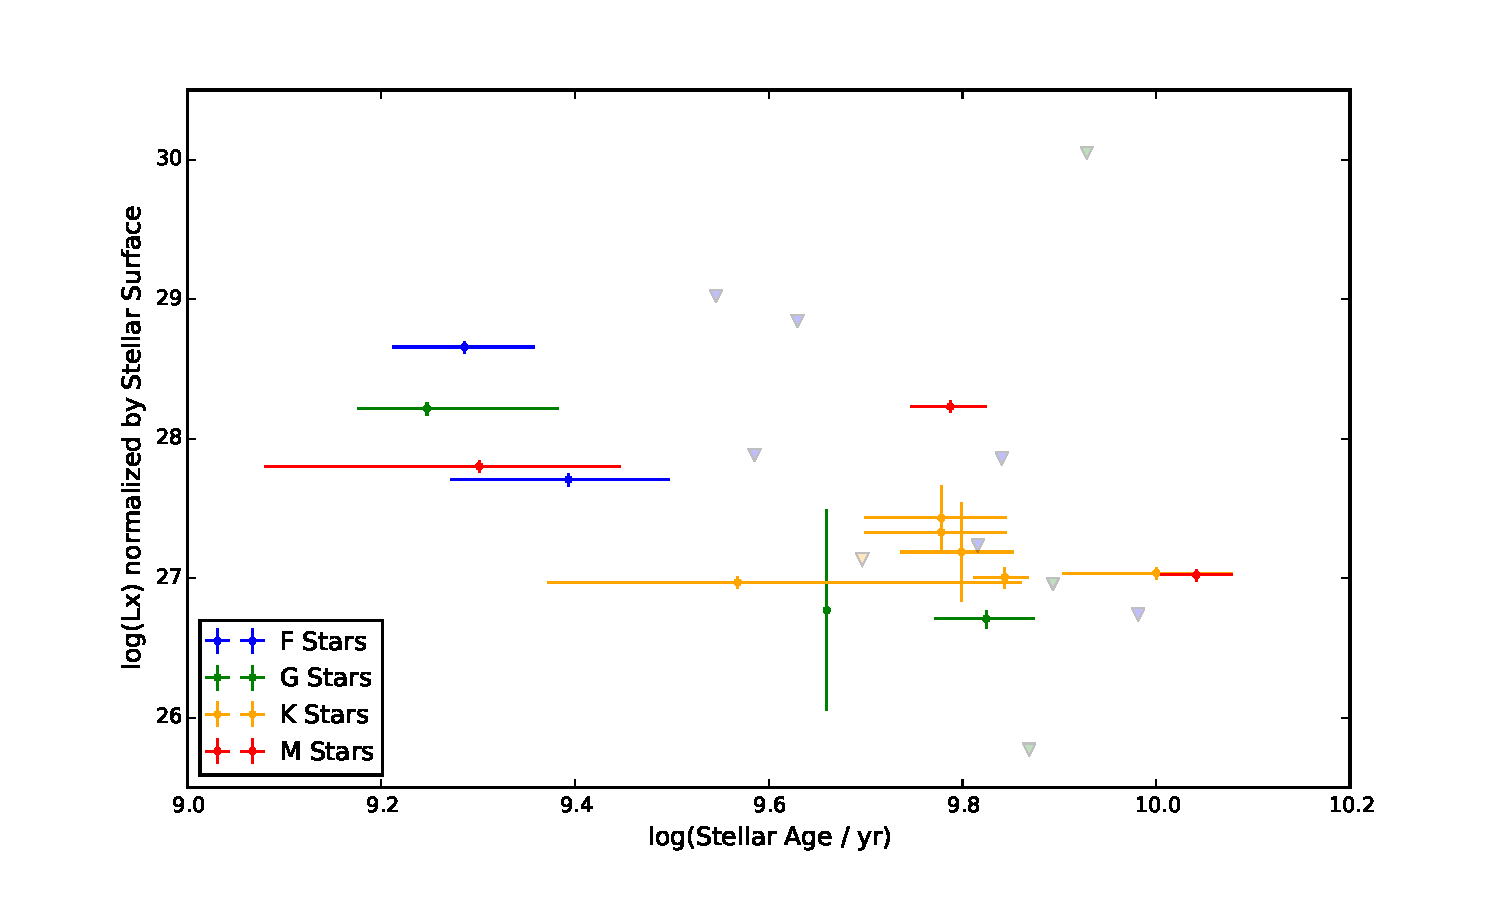
\includegraphics[scale=0.55]{Figures/3-Xray_age/xray_results.pdf}
    \caption[Plot of normalised X-ray luminosity as a function of age]{Logarithmic plot of normalised X-ray Luminosity as a function of stellar age for the data analysed in this work; specifically, the quantity on the vertical axis is $\log\frac{L_{x}}{(R_\ast/R_\odot)^{2}}$. Upper limits are indicated by downward triangles and lighter colours.}
    \label{fig:Xray_sample}
\end{figure}

The majority of the sample stars have asteroseismic ages, only eight of the sample have ages determined from other methods such as isochrone placement, white dwarf cooling times or association with a sub-population of stars in the galaxy. Ten stars in the sample have upper limits to their X-ray luminosities. The small number of X-ray detections demonstrates how difficult both the asteroseismic and X-ray measurements are. High-precision light-curves sampled at short cadences do not necessarily guarantee a precise measurement of age from asteroseismology. Even when a well-constrained age is determined, it does not guarantee an X-ray detection as resources are limited. Figure \ref{fig:Xray_sample} shows that the X-ray luminosity decreases with age as expected, but to gain more insight into what timescale this decrease occurs on the best-fitting relationship for the data was found.

Measurement errors are present in both the stellar age and the X-ray luminosity; therefore an orthogonal distance regression (ODR) \citep{Boggs_Rogers_1990} was performed to fit the logarithmic X-ray luminosity (normalised by stellar surface) against the stellar age. In a standard linear regression, the aim is to predict the y value from the x value and errors are only considered in the y direction. In the ODR method, errors in both x and y parameters are considered and thus the best-fitting relations obtained with this method are more reliable. In order to have normalised X-ray luminosities with familiar values, the stellar surface was normalised not in units of centimetres, but relative to the solar surface. This leads to normalised X-ray luminosities around $10^{27}$~erg\,s$^{-1}$\,$R_\odot^{-2}$. Only the 14 stars with X-ray detections or known X-ray luminosities were considered in this fit; for fitting purposes, we used symmetric errors in age and in $\log L_{\mathrm{X}}$. The best-fitting relationship obtained for the sample of stars in this work is shown in Equation \ref{Eq:best_fit_xray_age}. The best-fitting relationship is displayed visually in Figure \ref{fig:full_xray_plot_with_clusters}.

\begin{equation}
	\log\frac{L_{x}}{(R_\ast/R_\odot)^{2}} = 54.65 \pm 6.98 - (2.80 \pm 0.72)\log t
	\label{Eq:best_fit_xray_age}
\end{equation}

\begin{figure}[h]
    \centering
    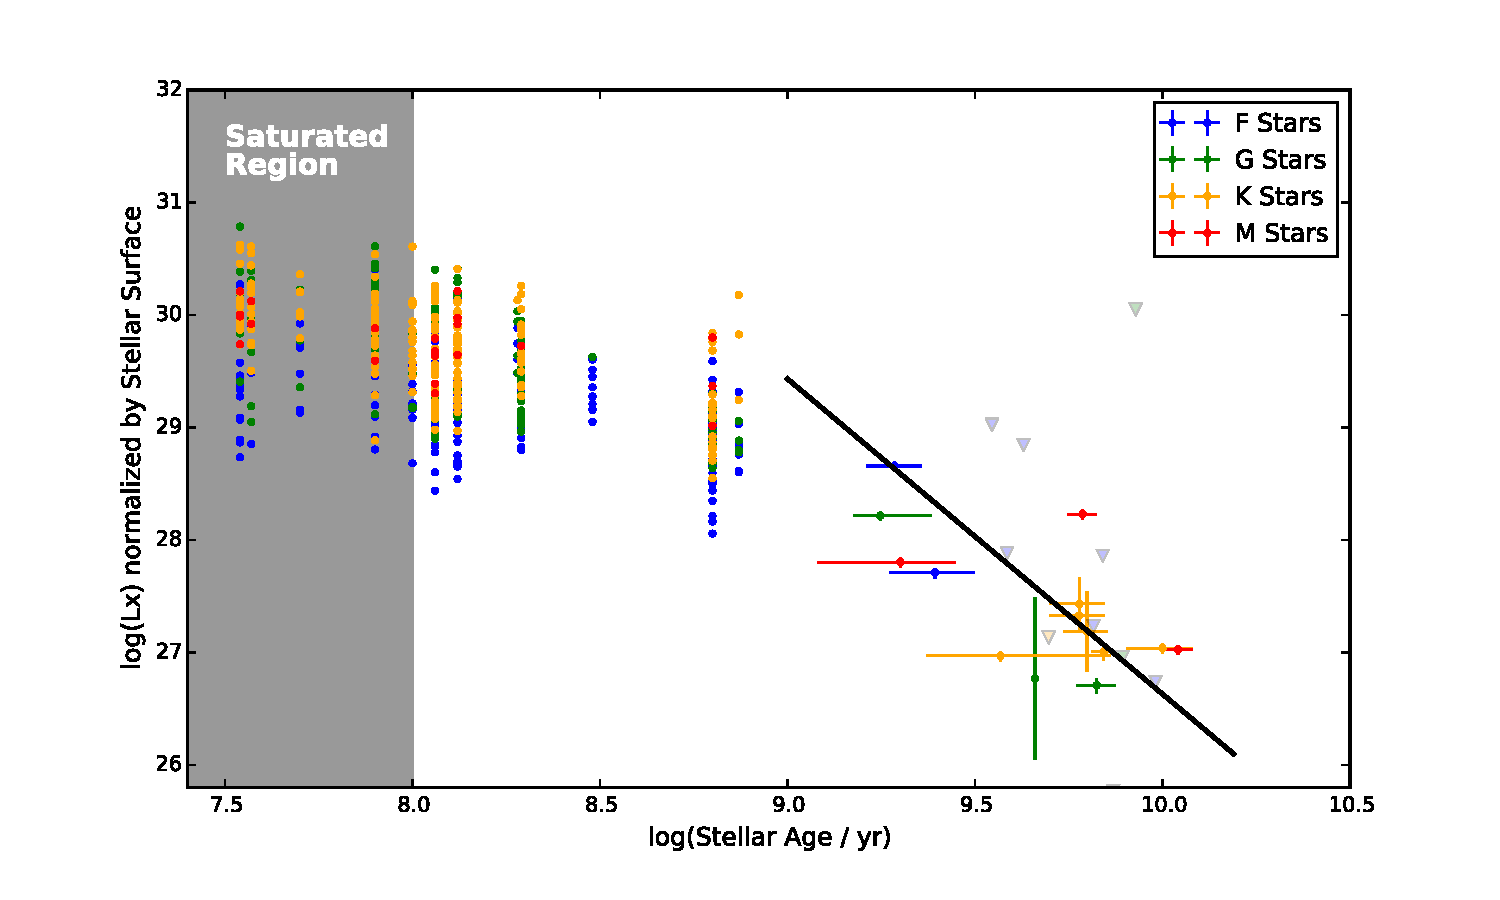
\includegraphics[scale=0.55]{Figures/3-Xray_age/full_xray_results.pdf}
    \caption[Plot of X-ray sample with best-fitting relationship and cluster data for reference]{Plot showing the data analysed in this work alongside the cluster data from \citet{Jackson_etal_2012}. The quantity on the vertical axis is $\log\frac{L_{x}}{(R_\ast/R_\odot)^{2}}$. Upper limits are indicated by downward triangles and lighter colours.  Black line indicates the best fit age-activity relationship found for data analysed in this work.}
    \label{fig:full_xray_plot_with_clusters}
\end{figure}

\section{Discussion}
Figure \ref{fig:full_xray_plot_with_clusters} shows the cluster data from \citet{Jackson_etal_2012} for ages below one gigayear, which were normalised by stellar surface area based on spectral type, alongside the sample of stars from this research for ages above one gigayear with our best-fitting age-activity relationship shown in black. As has been reported in many studies \citep{Vilhu_1984,Jardine_Unruh_1999,Pizzolato_etal_2003}, for very young stars there is a saturation of the X-ray luminosity until approximately 100 Myr when the X-ray luminosity starts to decay. \citet{Jackson_etal_2012} quantitatively investigated the age-activity relationship using clusters as calibrators, normalising by the bolometric luminosity and splitting into several mass bins. They found slope values for the age-activity relationship ranging from $-1.09 \pm 0.28$ to $-1.40 \pm 0.11$, considering seven spectral bins across the range from F-type stars to early M-type stars. Comparing these values to the slope value found in this work of $-2.80 \pm 0.72$, we find a steeper slope for the age-activity relationship at old ages than what is reported for any of the spectral bins for the younger stars. This steepening indicates a more rapid decay of stellar activity with age for cool stars older than a gigayear than for younger stars.

While there are a number of X-ray luminosity-age studies published in the literature, they tend to be focused on ages younger than a gigayear. The only comparable study for the relationship found in this work originates from \citet{Mamajek_Hillenbrand_2008} (henceforth MH08). MH08 derived an age-activity relationship for chromospheric activity derived from Ca~II H\&K emission. They also transform this into a relationship between X-ray luminosity and age, using a scaling relationship between chromospheric Ca~II H\&K and coronal X-ray emission, but no actual X-ray measurements of the sample stars were used. When the $L_{x}$ ages derived from the age-activity relationship from MH08 are compared to the literature ages for our sample, the MH08 $L_{x}$ ages tended to be somewhat younger than the literature ages. Two factors may come into play here: the relationship between $R'_{HK}$ and X-ray luminosity in MH08 used very few stars which are less active than $\log R'_{HK} \approx -5$. Our sample contains very old stars which we would expect to have chromospheric activity levels less than  $\log R'_{HK} \approx -5$, therefore probing a different part of the age/activity range than considered in the MH08 sample. Additionally, the use of their scaling relation between chromospheric and X-ray emission, which had been derived by \citet{Sterzik_Schmitt_1997} for stars with activity levels $\log R'_{HK} > -5$ , may not fully catch the actual relation of those emissions for very old and inactive stars.

We will now discuss the implications of the steepening of the age-activity relationship observed in this work in relation to stellar spin-down and activity decrease in general. As mentioned previously the rotational velocity of a star will decrease over time as a result of magnetic braking where the rotation is related to the time (or age) by $v_{rot} \propto t^{-\alpha}$ where $\alpha = 0.5$ \citep{Skumanich_1972,Meibom_etal_2011}. The first study of the relationship between rotation and activity was by \citealp{Pallavicini_etal_1981} who found that $L_{x} \propto (vsin(i))^{1.9}$. Observations of solar-like stars confirmed that the relationship between activity and rotation takes the form of $L_{x} \propto v_{rot}^{\beta}$ where $\beta \approx 2$ \citep{Pizzolato_etal_2003}. From these two relationships one can predict how X-ray luminosity varies with time as shown in Equation \ref{Eq:expected_theory_lx}.

\begin{equation}
	L_{x} \propto t^{-\alpha\beta} \text{\space where \space} \alpha\beta \approx 1
	\label{Eq:expected_theory_lx}
\end{equation}

Some previous studies have investigated the value of $\alpha\beta$. For example, \citealp{Gudel_etal_1997} studied nine solar-like G stars with ages ranging from 70 Myr to 9 Gyr (however they were constrained to rotation-inferred ages for most stars with ages beyond one gigayear) and found the value to be 1.5 for ages greater than 100 Myr. Later studies included \citealp{Giardino_etal_2008} that studied the 1.5 Gyr NGC 752 cluster and presented results that were consistent with a value for $\alpha\beta$ of 1.5, but also found evidence for a steepening of the X-ray luminosity scaling law after the age of the Hyades cluster (625 million years). However, \citealp{Feigelson_etal_2004} found an excellent fit for their data with a value for $\alpha\beta$ of 2 but also could not rule out the predicted value due to the small sample and systematic uncertainties.

The results from this research indicate that the value of $\alpha\beta$ for stars older than a gigayear is $2.80 \pm 0.72$, which is larger than the expected value of unity, and more in line with the direct investigations of $L_X$ versus age in the studies discussed in the previous paragraph. This leaves the challenge of explaining why the decay of magnetic activity is faster than predicted. One possibility is that the rotational spin down could be more rapid than expected from constant magnetised stellar winds \citep{Kawaler_1988}, i.e.\ $\alpha$ has a value greater than 0.5. \citet{Feigelson_etal_2004} also postulated that the coronal mass ejections may contribute to stellar angular deceleration, changing the alpha exponent. But a recent study by \citet{van_Saders_etal_2016} reports that there is weakened magnetic breaking for older late-type stars. Unfortunately, their sample and ours do not have sufficient overlap to compare age, rotation, and activity all together. A recent theoretical model by \citet{Blackman_Owen_2016} predicts weakened magnetic braking for older late-type stars; their model suggests that conductive losses are more important for these stars than wind losses which would imply a reduced angular momentum loss. Other theoretical work includes \citet{Garraffo_etal_2015} and \citet{Vidotto_etal_2016}, which show that the rotational spin down of a star may depend on the magnetic field geometry. If the rotational spin down was the only factor to affect the age-activity relationship then it should also show weakened magnetic braking and the exponent of the relationship should decrease and not increase as found in this work. From this evidence one would disfavour the more rapid rotational spin down as the cause of the more rapid decay of the magnetic activity.

Another possible explanation for the increased decay in magnetic activity for stars older than a gigayear is that the relationship between the X-ray luminosity and rotational velocity is not constant, i.e. the $\beta$ term changes as the star ages. There is some evidence for the steepening of the activity-rotation relationship, \citet{Wright_etal_2011} considered a small, unbiased subset of their large sample of solar and late-type stars and found that a value for $\beta$ of 2.7 was a better fit for their data than the generally accepted value of 2. This was in agreement with \citet{Gudel_etal_1997} who found a value for $\beta$ of 2.64 for a sample of nine solar analogs and \citet{Feigelson_etal_2004} who found an unexpectedly steep decay of X-ray emission as a function of age which could indicate a steepening of the activity-rotation relationship. However, more research is needed into the activity-rotation relationship to confirm if there is a steepening of the relationship as one of the lowest values considered in the \citet{Wright_etal_2011} subset of data was of the Sun. In this research older stars have been considered that have lower X-ray luminosities than the Sun therefore the activity-rotation relationship needs to be extended to lower X-ray luminosities.

An important caveat about using the X-ray luminosity as a magnetic activity indicator is that many stars display activity cycles and thus the X-ray luminosity can vary by orders of magnitude depending on the phase of the activity cycle as seen in the solar values used in this work. Where possible, the variation of the X-ray luminosity due to magnetic activity cycles has been incorporated into the errors adopted in this work (e.g. Sun, 61 Cyg A and $\alpha$ Cen B). However, long term monitoring is required which is not available for most stars. Further improvement on the age-activity relationship would include a full sample of stars with long-term averages for X-ray luminosity which would not only increase the reliability of the relationship found but also increase the confidence of any ages determined from the relationship.

\section{Conclusions}
In this work we have presented new X-ray detections of several old cool stars together with an analysis of archival data to form a sample of 24 cool stars with ages beyond one gigayear. Most of the stellar ages in the sample have been determined by asteroseismology, providing more accurate ages for old stars than most other studies were able to provide. We have investigated the age-activity relationship of these stars using observations from the \Chandra and \XMM X-ray telescopes. X-ray luminosities were determined for fourteen stars primarily, and spectral modelling was performed for eight of those stars; upper limits to the X-ray luminosity were determined for a further ten stars. The X-ray luminosity of the sample stars was normalised by the stellar surface, in order to  perform an analysis across varying spectral types. An age-exponent value of $\alpha\beta = 2.80 \pm 0.72$ was found, which represents a steepening of the age-activity relationship compared to what is seen for stars in clusters with ages below one gigayear. A possible explanation for this steepening of the age-activity relationship is that rotational spin down is more rapid than previously thought. However, a recent observational study \citep{van_Saders_etal_2016} indicates that there is weakened magnetic braking for older cool stars. If this is indeed true, our data presents evidence that there is a strong steepening of the rotation-activity relationship at old stellar ages instead of the age-rotation relationship itself. In either case, the data we have presented here demonstrates that the relationship between stellar age and activity steepens towards old stellar ages. Combined studies of age, rotation, and activity will be able to shed light on which components of the relationship are responsible for this.

\newpage